\chapter{Meccanica dei Rigidi}
\section{Sistema rigido e DOF}
Si definisce sistema rigido, un sistema materiale $\mathfrak{R}$, dotato di una massa $M$ i cui punti mantengono invariata la reciproca distanza durante il moto. La \emph{proprietà di rigidità} per un sistema composto da $n$ punti materiali può essere espressa nel seguente modo,
\begin{equation}
	\vert P_i - P_j\vert = d \in \mathbb{R},\quad \forall i,j = 1,2, \cdots, n
\end{equation}
descriviamo la massa per corpi rigidi con densità \emph{discreta} e \emph{continua},
\begin{equation}
	M = \sum_{i = 1}^{n} m_i  \qquad M = \int_{V_{\mathfrak{R}}} \rho dV
\end{equation}
con $\rho$ \emph{densità} della particella di volume infinitesimo $dV$.

\paragraph{}
Indichiamo con $\mathfrak{R_n}$ un sistema rigido composto da $n$ punti nello spazio. Descriviamo i gradi di libertà (Degree Of Freedom DOF) come il numero di variabili che servono per descrivere la \emph{\textbf{posa}} (\emph{posizione} + \emph{orientamento}) del corpo. Otteniamo quindi:
\begin{itemize}
	\item $\mathfrak{R_1}$: un sistema con un solo punto ha $3$ DOF.
	\item $\mathfrak{R_2}$: un sistema con due punti ha apparentemente $6$ DOF ma essendo rigido, il vincolo impone che due variabili sono uguali, pertanto ha $5$ DOF.
	\item $\mathfrak{R_3}$: un sistema con tre punti ha $9$ variabili e $3$ vincoli, pertanto ottengo $6$ DOF, la cosa interessante è che qualsiasi sistema rigido con più di 3 punti ha comunque tanti vincoli che riconducono fino a $6$ DOF.
\end{itemize}

\section{Cinematica}
\paragraph{}
La descrizione cinematica di un rigido si articola considerando due SdR:
\begin{itemize}
	\item Fisso $\Sigma$: $\lbrace\Omega, \underline{a}, \underline{b}, \underline{c}\rbrace$
	\item Solidale al rigido $S$: $\lbrace O, \underline{i}, \underline{j}, \underline{k} \rbrace$
\end{itemize} 
\begin{center}
	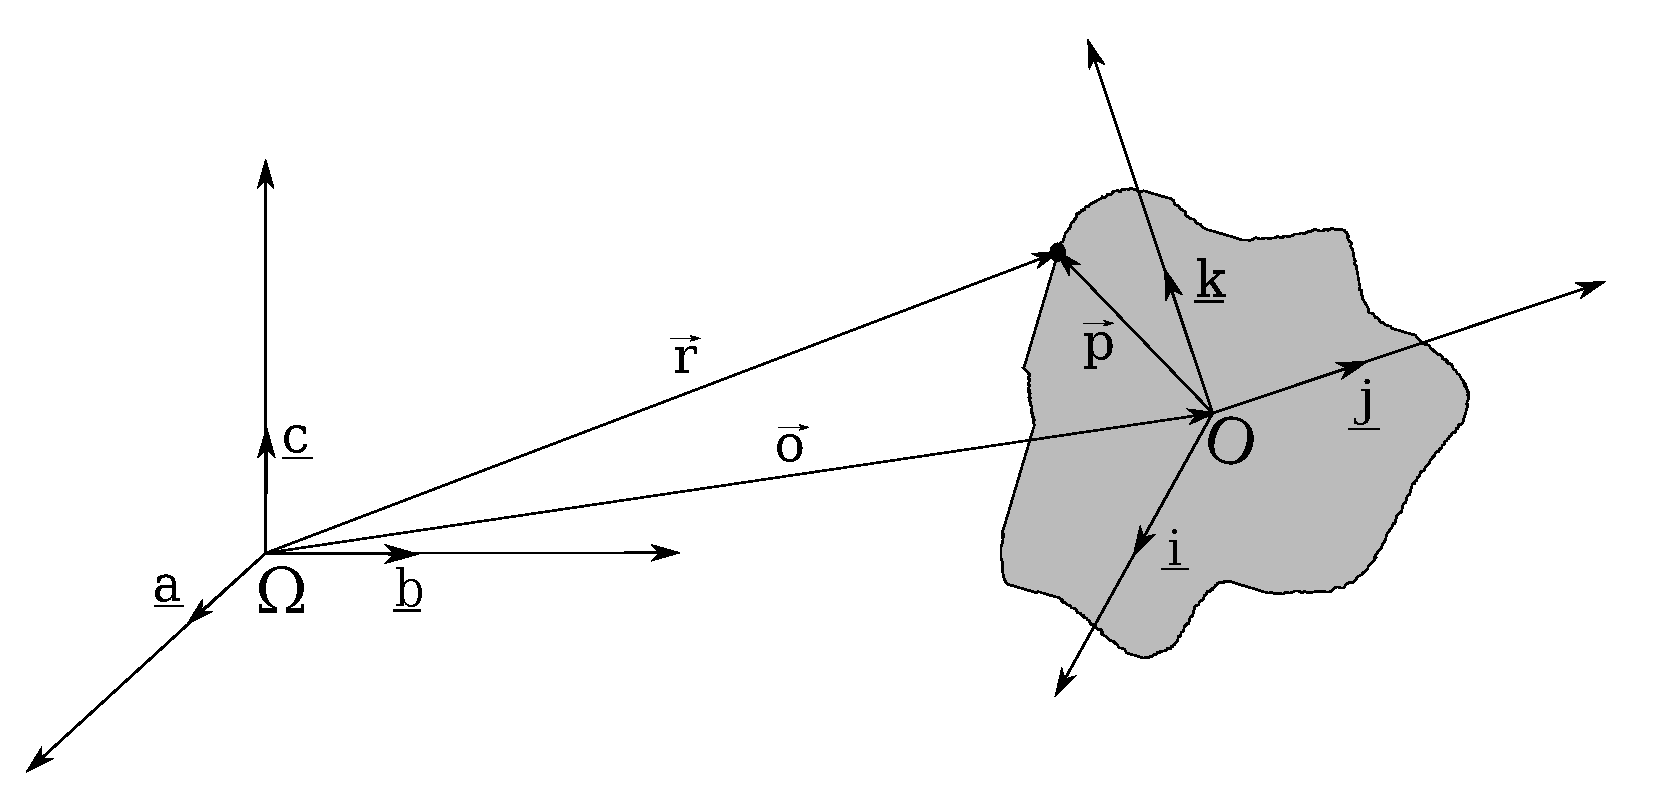
\includegraphics[scale=0.4]{SdRRigido.pdf}
	\caption{SdR fisso e solidale.}
\end{center}
in generale, per un punto $P$ nello spazio, valgono le seguenti relazioni di cinematica relativa:
\begin{equation}
	\begin{cases}
		\vec{r} = \vec{o} + \vec{p} \\
		\vec{v}_{P,\Sigma} = \vec{v}_{O,\Sigma} + \vec{v}_{P,S} + \vec{\omega} \times \vec{p} \\
		\vec{a}_{P,\Sigma} = \underbrace{\vec{a}_{O,\Sigma} + \vec{\omega} \times (\omega \times \vec{p}) + \dot{\vec{\omega}} \times \vec{p}}_{\vec{a}_{T}} + \underbrace{2\vec{\omega} \times \vec{v}_{P,S}}_{\vec{a}_{C}} + \vec{a}_{S} \\
	\end{cases}
\end{equation}
adesso, consideriamo che tra i punti di un corpo rigido (composto da $n$ punti) vale la \emph{proprietà di rigidità} $\vert P_i - P_j\vert = d \in \mathbb{R},\quad \forall i,j = 1,2, \cdots, n$ con $d$ costante, pertanto per l'osservatore non inerziale $S$ tutti i punti del corpo rigido sono fermi. Quindi, le equazioni $(C.3)$ diventano:
\begin{equation}
	\begin{cases}
		\vec{r} = \vec{o} + \vec{p} \\
		\vec{v}_{P,\Sigma} = \vec{v}_{O,\Sigma} + \vec{\omega} \times \vec{p} \\
		\vec{a}_{P,\Sigma} = \vec{a}_{T} \\
	\end{cases}
\end{equation}
inoltre, notiamo come la formula della velocità del punto si possa, in via del tutto generale proiettare sul vettore $\vec{\omega}$ e ottenere la seguente composizione,
\begin{equation}
	\vec{v}_{P,\Sigma} = (\vec{v}_{P,\Sigma})^{\,\parallel} + (\vec{v}_{P,\Sigma})^{\,\perp}
\end{equation}
che ci permette di distinguere i vari tipi di moto:
\begin{itemize}
	\item Se $\vec{\omega} = \vec{0}$ il moto è \emph{traslatorio} con $3$ DOF.
	\item Se $\vec{v}_{O,\Sigma} = \vec{0}$ abbiamo due possibilità:
	\begin{itemize}
		\item In generale se $\vec{\omega}$ è libero di muoversi, il moto è di \emph{precessione} con $3$ DOF.
		\item Se $\vec{\omega}$ ha direzione costante, il moto è di \emph{rotazione} con $1$ DOF.
	\end{itemize}		
	\item Se $(\vec{v}_{P,\Sigma})^{\,\parallel} \neq \vec{0}$ il moto è \emph{elicoidale} con $2$ DOF.
	\item Se $(\vec{v}_{P,\Sigma})^{\,\parallel} = \vec{0}$ il moto è \emph{rigido piano} con $3$ DOF.
\end{itemize}

\subsubsection{Spostamento elementare}
Possiamo esprimere lo \emph{spostamento elementare} di un punto qualsiasi del corpo rigido attraverso la \textbf{legge fondamentale della cinematica} per sistemi rigidi. Infatti, supponiamo di voler calcolare la velocità del punto $P$ e del punto $Q$,
\begin{center}
	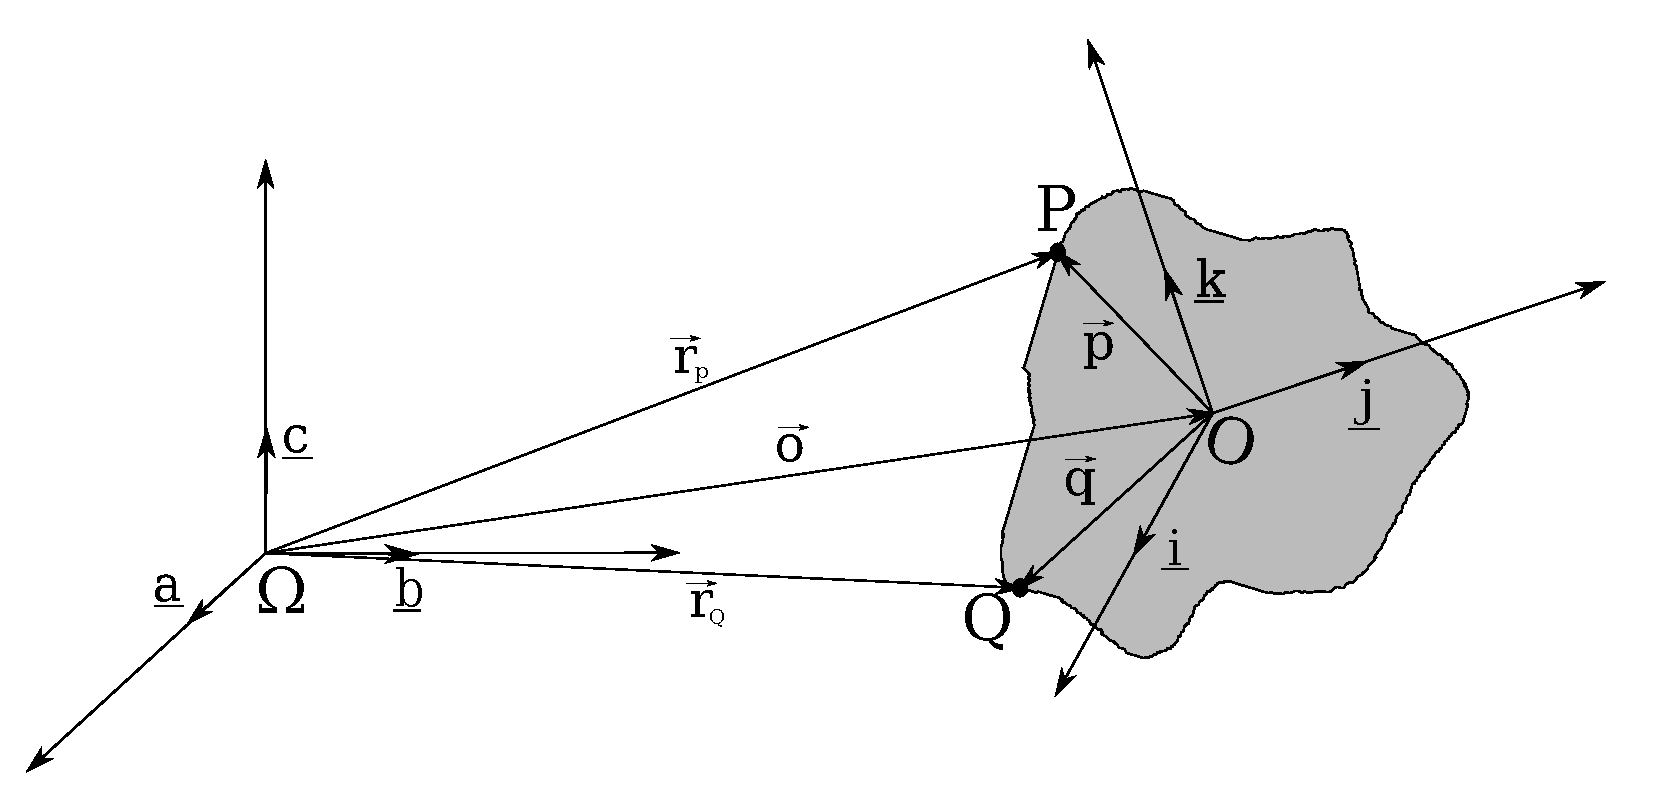
\includegraphics[scale=0.3]{LeggeCinRig.pdf}
	\caption{Legge fondamentale della cinematica.}
\end{center}
otteniamo, 
\begin{equation}
	\vec{v}_{P,\Sigma} = \vec{v}_{O, \Sigma} + \vec{\omega} \times \vec{p} 
	\qquad \qquad
	\vec{v}_{Q,\Sigma} = \vec{v}_{O, \Sigma} + \vec{\omega} \times \vec{q} 
\end{equation}
e considerando il vincolo di rigidità imposto dalla $(C.1)$, avremo
\begin{equation*}
	\vec{v}_{P,\Sigma} - \vec{v}_{Q,\Sigma} = \vec{0} \quad \Rightarrow \quad \vec{v}_{P,\Sigma} - \vec{v}_{Q,\Sigma} = \vec{v}_{O, \Sigma} + \vec{\omega} \times \vec{p} - \vec{v}_{O, \Sigma} - \vec{\omega} \times \vec{q} = \vec{0}
\end{equation*}
e otteniamo 
\begin{equation}
	\vec{v}_{P,\Sigma} = \vec{v}_{Q,\Sigma} + \vec{\omega} \times (\vec{p} - \vec{q})
\end{equation}

A questo punto, possiamo calcolare lo spostamento elementare $d\vec{p}$ come 
\begin{equation}
	d \vec{p} = \dot{\vec{p}} dt = (\dot{\vec{q}} + \vec{\omega} \times (\vec{p} - \vec{q}))dt
\end{equation}
che esplicitando il secondo membro attraverso la moltiplicazione col $dt$ si ottiene,
\begin{equation}
	d\vec{p} = d\vec{q} + \vec{\omega}dt \times (\vec{p} - \vec{q})
\end{equation}
ottenendo lo \textbf{\emph{spostamento elementare}} di un punto $P$ del corpo rigido $\mathfrak{R}$ nell'intervallo di tempo $(t, t+dt)$.
\section{Dinamica}
Da ora in avanti, per semplificare la notazione consideriamo il sistema $\lbrace O, \underline{i}, \underline{j}, \underline{k} \rbrace$ come la \emph{terna fissa} e il corpo rigido come oggetto nello spazio. Sarà interessante e molto utile identificare la \emph{terna baricentrica} al corpo come la \emph{terna solidale}. Quindi non ci riferiremo più alla figura C.1, ma avremo un'altra rappresentazione del tutto generica mostrata a figura C.3.   
\subsubsection{Centro di massa}
Immaginiamo il corpo come un numero infinito di particelle, ognuna dotata di una frazione infinitesima della massa totale del corpo. Possiamo calcolare quindi, la posizione del \emph{centro di massa (o baricentro)}.
\begin{equation}
	\vec{p}_{CM} = \frac{1}{\int_{V} \rho dV} \int_{V} \vec{p} \rho dV 
\end{equation} 
dove $\vec{p}$ denota il vettore delle coordinate che individua la posizione dell'elemento di volume infinitesimo. 

Se il sistema rigido ha una \emph{distribuzione discreta} formata da esattamente $n$ punti con massa $m_i$, possiamo riscrivere la $(C.10)$ nel modo seguente,
\begin{equation}
	\vec{p}_{CM} = \frac{1}{\sum_{i = 1}^{n} m_i} \sum_{i = 1}^{n} m_i \vec{p}_i
\end{equation}.
\subsubsection{Momento di inerzia}
Il momento di inerzia di un punto materiale o di un corpo rigido è una grandezza che esprime l'inerzia dei corpi rispetto ai moti rotazionali, ossia la tendenza a opporsi alle rotazioni, esattamente come la massa nei moti di traslazione.
\begin{center}
	\includegraphics[scale=0.3]{momentoInerzia.pdf}
	\caption{SdR \emph{fisso}.}
\end{center}
\paragraph{}
Consideriamo un volumetto del corpo rigido di massa $\rho dV$ individuato dal vettore $\vec{p}$ ed un asse $r$. Sia $d$ la distanza del volumetto dall'asse. Definiamo \emph{momento di inerzia} del volumetto rispetto all'asse la quantità:
\begin{equation}
	I_r = d^2 \rho dV
\end{equation}
quindi, per estensione, il \emph{momento d'inerzia del corpo} di massa $M$, volume $V$ e densità $\rho$ rispetto all'asse $r$ è definito come
\begin{equation}
	I_r = \int_{V_{\mathfrak{R}}} d^2 \rho dV
\end{equation}
chiaramente la \emph{distanza} $d$ è dipendente dal vettore posizione $\vec{p}$ e quindi sarebbe più opportuno scrivere $d = d(\vec{p})$.

Adesso consideriamo $\underline{r}$ il versore della retta $r$ e utilizzando l'operatore $S(\cdot)$, possiamo scrivere il \emph{momento di inerzia} del rigido $\mathfrak{R}$ rispetto alla retta $r$ passante per $O$ come,
\begin{equation}
I_r = \underline{r}^T \underbrace{\Biggl( \int_{V_{\mathfrak{R}}} S^T(\vec{p}) S(\vec{p}) \rho dV \Biggr)}_{I_o} \underline{r} = \underline{r}^T I_O \underline{r}
\end{equation}
pertanto otteniamo il \emph{tensore di inerzia} $I_O$ del corpo $\mathfrak{R}$ relativo al polo $O$,
\begin{equation*}
	I_O = 
	\begin{bmatrix}
		\int_{V_{\mathfrak{R}}} (p_y^2 + p_z^2) \rho dV & - \int_{V_{\mathfrak{R}}} p_xp_y \rho dV & - \int_{V_{\mathfrak{R}}} p_xp_z \rho dV \\
		- \int_{V_{\mathfrak{R}}} p_xp_y \rho dV & \int_{V_{\mathfrak{R}}} (p_x^2 + p_z^2) \rho dV & - \int_{V_{\mathfrak{R}}} p_yp_z \rho dV \\
		- \int_{V_{\mathfrak{R}}} p_xp_z \rho dV & - \int_{V_{\mathfrak{R}}} p_yp_z \rho dV & \int_{V_{\mathfrak{R}}} (p_x^2 + p_y^2) \rho dV
	\end{bmatrix}
	= 
	\begin{bmatrix}
		I_{xx} & -I_{xy} & -I_{xz} \\
		- I_{xy} & I_{yy} & -I_{yz} \\
		-I_{xz} & -I_{yz} & I_{zz} \\
	\end{bmatrix}
\end{equation*}
con:
\begin{itemize}
	\item $I_{xx}$, $I_{yy}$, $I_{zz}$ sono i \textbf{momenti di inerzia} di $\mathfrak{R}$ rispetto al sistema solidale $S$.
	\item $I_{xy}$, $I_{xz}$, $I_{yz}$ sono i \textbf{momenti centrifughi} di $\mathfrak{R}$ rispetto alle coppie di piani ordinati ($xy$, $xz$, $yz$).
\end{itemize}

Il \emph{tensore di inerzia} dipende sia dal polo che dall'orientamento della terna di riferimento. Se si considera una nuova terna, ruotata secondo la matrice $R$ rispetto alla terna originaria, il tensore si scrive: $I_O' = RI_OR^T$.

Dal momento che il tensore di inerzia è una matrice simmetrica e \emph{definita positiva}, applicando il teorema spettrale esiste sempre una terna di riferimento in cui il tensore di inerzia assume la forma diagonale. Tale terna è detta \textbf{terna principale di inerzia} relativa al polo $O$. Inoltre, se $O \equiv CM$ allora si parla di \textbf{terna centrale di inerzia}.

\subsubsection{Huygens-Steiner}
Sia $I_{CM}$ il momento di inerzia di un corpo di massa $M$ rispetto ad un asse passante per il baricentro. Consideriamo un asse parallelo ma passante per $O$ e $d$ la distanza tra i due assi, allora possiamo scrivere
\begin{equation}
	I_O = I_{CM} + Md^2
\end{equation}  
\begin{center}
	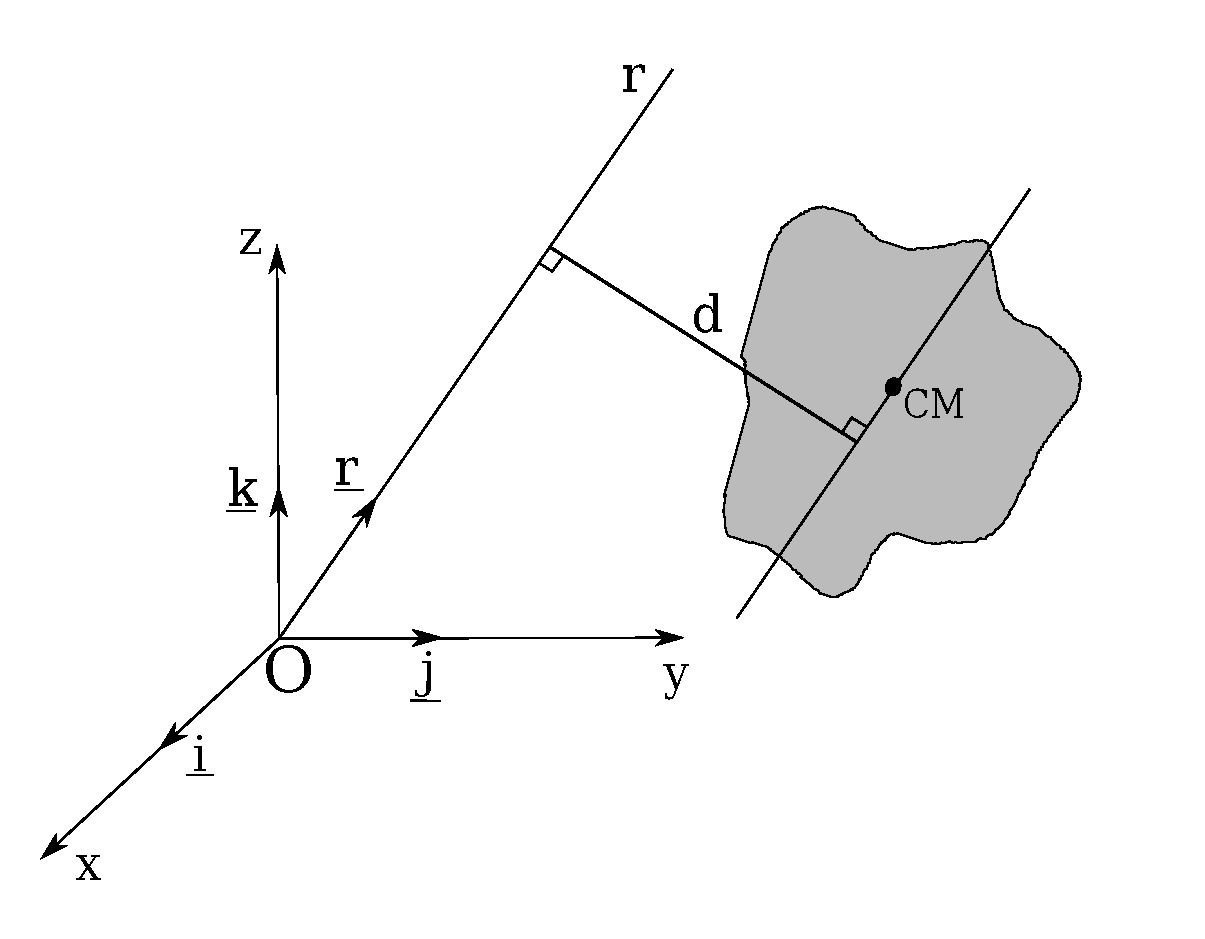
\includegraphics[scale=0.3]{HuygensSteiner.pdf}
	\caption{Teorema classico di Steiner.}
\end{center}
e questo era il classico teorema di Huygens-Steiner, ma passando ai tensori otteniamo il seguente risultato. Sia $I_{CM}$ il tensore di inerzia del corpo di massa $M$ rispetto ad una terna avente come origine il baricentro. 
\begin{center}
	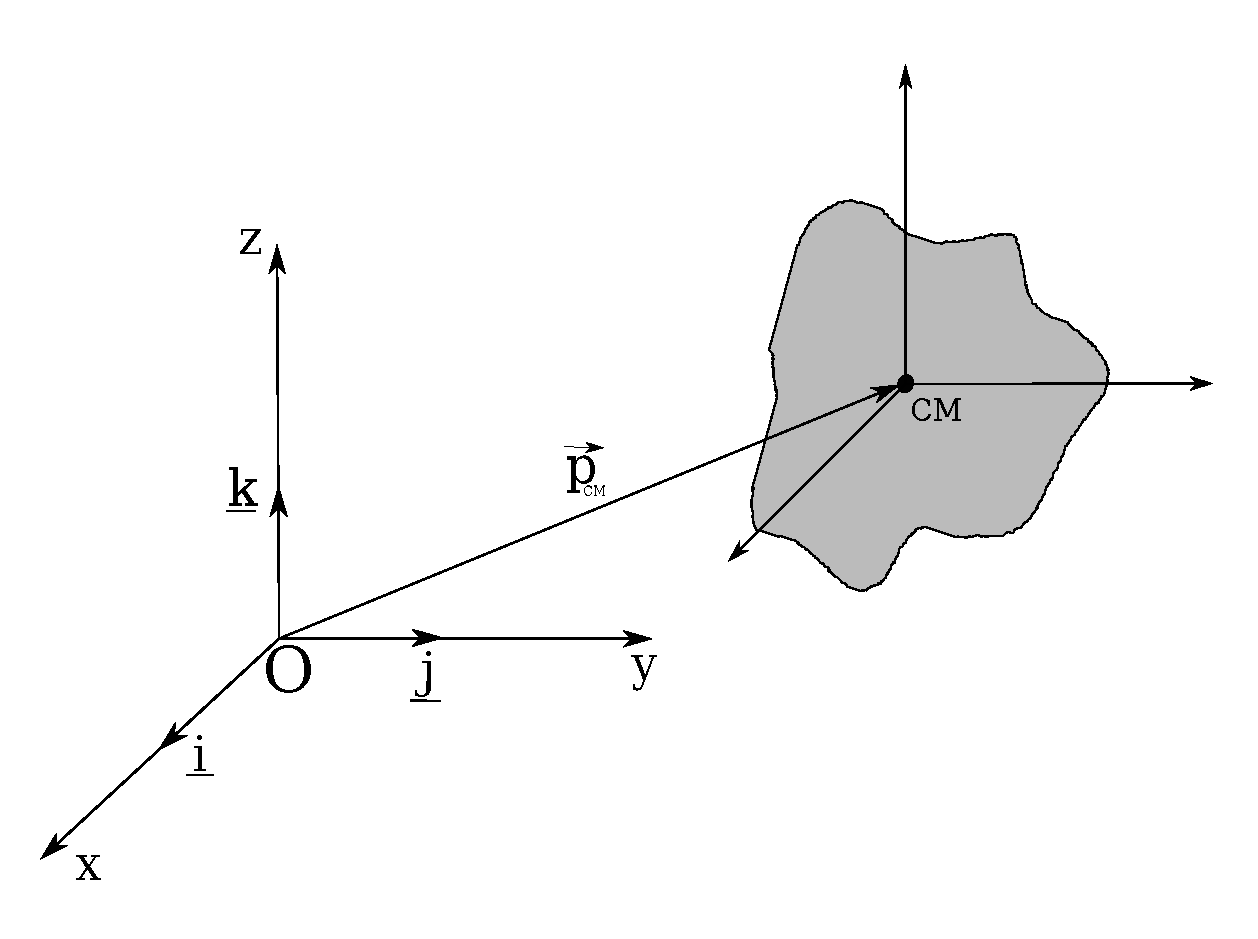
\includegraphics[scale=0.3]{HuygensSteinerTensori.pdf}
	\caption{Terna fissa e terna baricentrica.}
\end{center}

Il tensore di inerzia, rispetto ad una terna parallela a quella baricentrale e avente origine in un diverso punto $O$, è dato da
\begin{equation}
	I_O = I_{CM} + M S^T(\vec{p}_{CM})S(\vec{p}_{CM})
\end{equation}


\subsubsection{Momento angolare}
Sia $\dot{\vec{p}}$ la velocità della generica particella di $\mathfrak{R}$ di massa elementare $\rho dV$ nella terna $\lbrace O, \underline{i}, \underline{j}, \underline{k} \rbrace$. Si definisce \textbf{quantità di moto} del corpo $\mathfrak{R}$ il vettore
\begin{equation}
	\vec{l} = \int_{V_{\mathfrak{R}}} \dot{\vec{p}} \rho dV = \frac{\int_{V_{\mathfrak{R}}} \rho dV}{\int_{V_{\mathfrak{R}}} \rho dV} \int_{V_{\mathfrak{R}}} \dot{\vec{p}} \rho dV = M \dot{\vec{p}}_{CM}
\end{equation}

Definiamo il \textbf{momento angolare}, in riferimento alla figura $(C.5)$, della particella rispetto al punto $O$ come il vettore,
\begin{equation}
	\vec{k}_O = \vec{p} \times \rho dV \dot{\vec{p}}
\end{equation}
e chiaramente estendendo il concetto a tutto il corpo otteniamo, 
\begin{equation}
	\vec{k}_O = \int_{V_{\mathfrak{R}}} \vec{p} \times \rho dV \dot{\vec{p}}
\end{equation}
e se scegliamo un generico punto dello spazio, come ad esempio $Q \neq O$, otteniamo
\begin{equation}
	\vec{k}_Q = \vec{q} \times \rho dV \dot{\vec{p}} = (\vec{p} - \vec{p}_q) \times \rho dV \dot{\vec{p}} 
\end{equation}
e quindi otteniamo il momento angolare del corpo $\mathfrak{R}$ relativo al polo $Q$ come il vettore
\begin{equation}
	\vec{k}_Q = \int_{V_{\mathfrak{R}}} (\vec{p} - \vec{p}_q) \times \rho dV \dot{\vec{p}}
\end{equation}
\begin{center}
	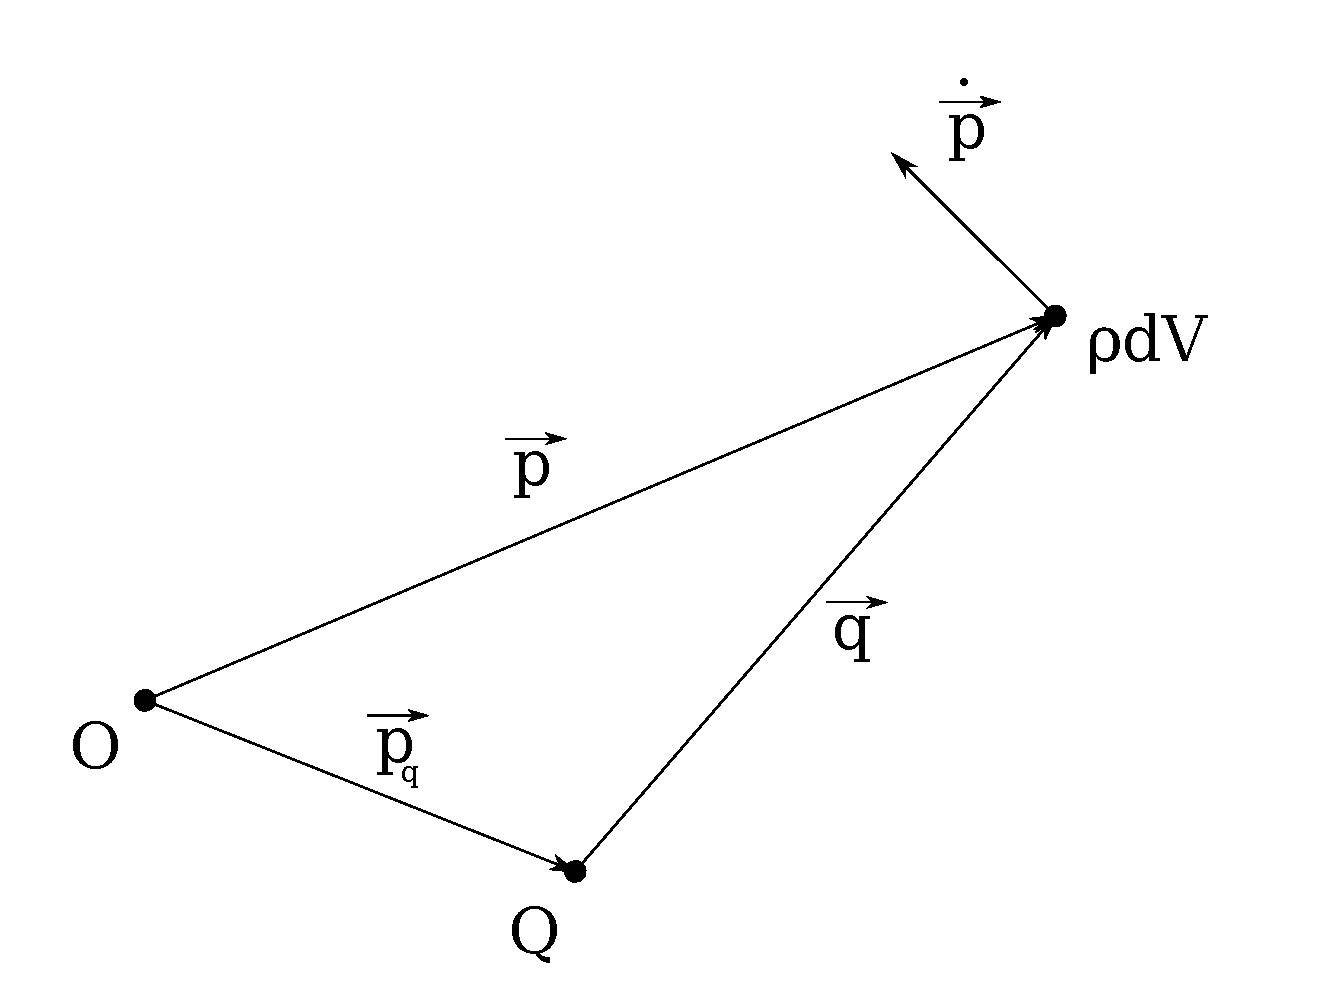
\includegraphics[scale=0.25]{momentoAngolare.pdf}
	\caption{Immagine di riferimento per il calcolo del momento angolare.}
\end{center}

Per i corpi rigidi, il momento angolare diventa il seguente,
\begin{equation}
	\vec{k}_Q = I_{CM} \vec{\omega} + (\vec{p}_{CM} - \vec{p}_Q) \times M \dot{\vec{p}}_{CM}
\end{equation}
con $I_{CM}$ il tensore di inerzia relativo al baricentro espresso in una terna con origine nel baricentro e parallela a quella di riferimento.

\subsubsection{Momento torcente}
Le \emph{forze} agenti su un generico sistema meccanico possono essere classificate nel modo seguente:
\begin{center}
	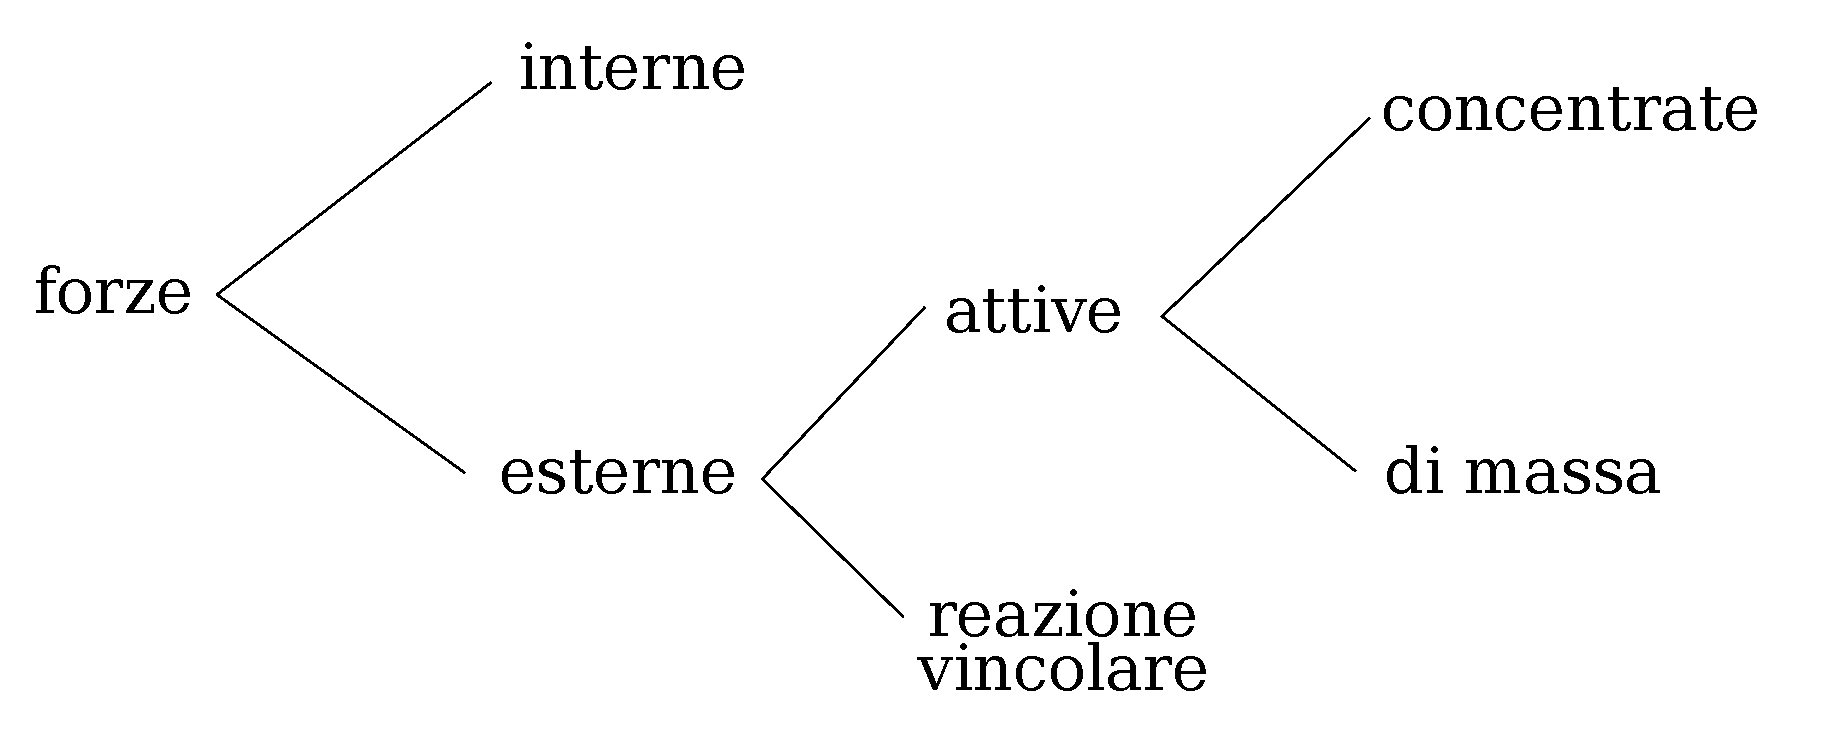
\includegraphics[scale=0.25]{classificazioneForze.pdf}
\end{center}
\begin{itemize}
	\item Le \emph{Forze interne}, sono quelle scambiati tra parti dello stesso sistema, hanno risultante e momento risultante nullo e non influenzano il moto del corpo rigido.
	\item Le \emph{Forze concentrate}, sono applicate in punti particolari del corpo rigido laddove le \emph{Forze di massa} agiscono su tutte le particelle elementari costituenti il corpo. Un esempio di forza di massa è la forza gravitazionale che per ciascuna particella è pari a $\vec{g} \rho dV$.
	\item Le \emph{Forze di reazione vincolare} sono quelle che si esplicano in seguito al contatto tra due o più corpi. Tali forze possono essere distribuite sulla superficie di contatto o da ritenersi concentrate.
\end{itemize}
\paragraph{}
Per un corpo rigido $\mathfrak{R}$ sottoposto alla forza gravitazionale e a forze attive e/o di reazione vincolare $f_1, f_2, \cdots, f_n$ concentrate nei punti $P_1, \cdots, P_n$, la \emph{risultante delle forze esterne} $\vec{f}$ e il \emph{momento torcente risultante} $\vec{\mu}_Q$ rispetto ad un polo $Q$ valgono:
\begin{eqnarray}
	\vec{f} = \int_{V_{\mathfrak{R}}} \vec{g} \rho dV + \sum_{i = 1}^{n} \vec{f}_i = M\vec{g} + \sum_{i = 1}^{n} \vec{f}_i \\
	\vec{\mu}_Q = \int_{V_{\mathfrak{R}}} (\vec{p} - \vec{p}_Q) \times \vec{g} \rho dV + \sum_{i = 1}^{n} (\vec{p}_i-\vec{p}_Q) \times \vec{f}_i = \\
	= (\vec{p}_{CM} - \vec{p}_Q) \times M\vec{g} + \sum_{i = 1}^{n} (\vec{p}_i-\vec{p}_Q) \times \vec{f}_i 
\end{eqnarray}

Supponendo di voler calcolare il momento risultante rispetto ad un altro polo $Q'$ avendo $\vec{f}$ e $\vec{\mu}_Q$ possiamo scrivere, in riferimento alla figura C.6,
\begin{center}
	\includegraphics[scale=0.28]{MomentoTorcente.pdf}
	\caption{Calcolo del momento torcente.}
\end{center}
\begin{equation}
	\vec{\mu}_{Q'} = \vec{\mu}_Q + (\vec{p}_Q - \vec{p}_{Q'}) \times \vec{f}
\end{equation}

\subsubsection{Equazioni cardinali}
Si consideri un generico sistema meccanico sottoposto a forze esterne di risultante $\vec{f}$ e momento risultante $\vec{\mu}_Q$. Il moto del sistema in una terna $S$ è governato dalle seguenti \emph{leggi fondamentali della dinamica}:
\begin{align}
	\dot{\vec{l}} = \vec{f} \\
	\dot{\vec{k}}_Q = \vec{\mu}_{Q}
\end{align} 
con $Q$ polo fisso o coincidente con il baricentro $CM$ del sistema. Per un sistema rigido a massa costante, la $(C.27)$ diventa \emph{l'equazione di Newton} e la $(C.28)$ diventa \emph{l'equazione di Eulero},
\begin{equation}
	\begin{cases}
		\vec{f} = M \ddot{\vec{p}}_{CM} \\
		\vec{\mu}_{Q} = I_Q \dot{\vec{\omega}} + \vec{\omega} \times (I_Q \vec{\omega}) 
	\end{cases}
\end{equation}.


\section{Lavoro ed energia}
\subsubsection{Lavoro}
Assegnata una forza $\vec{f}_i$ applicata in un punto di posizione $\vec{p}_i$ rispetto a una terna $\lbrace O, \underline{i}, \underline{j}, \underline{k} \rbrace$ si definisce \emph{lavoro elementare} della forza $\vec{f}_i$ nello spostamento $d\vec{p}_i$ lo scalare,
\begin{equation}
	dW_i = \vec{f}_i^{\,\,T} d\vec{p}_i
\end{equation}

Nel caso di un corpo rigido $\mathfrak{R}$ sottoposto a $\vec{f}$ e $\vec{\mu}_Q$ rispetto ad un qualsiasi punto $Q \in \mathfrak{R}$, il lavoro elementare nello spostamento rigido $(C.9)$ è espresso come, 
\begin{equation}
	dW = (\vec{f}^{\,\,T} \dot{\vec{p}}_Q + \vec{\mu}^{\,T}_Q \omega)dt = \vec{f}^{\,\,T} d\vec{p}_Q + \vec{\mu}_Q^{\,T} \vec{\omega} dt
\end{equation}
facendo attenzione alla notazione con la $(C.9)$, infatti, $\vec{p}_Q \equiv \vec{q}$.

\subsubsection{Energia cinetica}
Definiamo \emph{l'energia cinetica} di un volumetto di massa $\rho dV$ di $\mathfrak{R}$ individuato dal vettore $\vec{p}$ espresso in terna $\lbrace O, \underline{i}, \underline{j}, \underline{k} \rbrace$ come,
\begin{equation}
	T = \frac{1}{2} \underbrace{\rho dV}_{m} \underbrace{\dot{\vec{p}}^{\,\,T} \dot{\vec{p}}}_{\vert\vec{v}_{P}\vert^2}
\end{equation}
ed estendendo a tutto il corpo rigido otteniamo,
\begin{equation}
	T = \frac{1}{2} \int_{V_{\mathfrak{R}}} \dot{\vec{p}}^{\,\,T} \dot{\vec{p}} \rho dV
\end{equation}
che per i corpi rigidi, ha la seguente espressione notevole (teorema di \emph{Köenig}),
\begin{equation}
T = \frac{1}{2} M \dot{\vec{p}}_{CM}^{\,\,T} \dot{\vec{p}}_{CM} + \frac{1}{2} \vec{\omega}^{\,T} I_{CM} \vec{\omega}
\end{equation}
dove $\vec{p}_{CM}$ è la posizione del baricentro e $I_{CM}$ è il \textbf{tensore di inerzia} rispetto ad una terna con origine il baricentro e parallela alla terna di riferimento. Nel caso di \emph{rotazione attorno ad un asse fisso} coincidente con $z$, si riscrive la $(C.34)$ come
\begin{equation}
	T = \frac{1}{2} M \dot{\vec{p}}_{CM}^{\,\,T} \dot{\vec{p}}_{CM} + \frac{1}{2} (I_{CM})^{\parallel z} \omega_z^2
\end{equation}
dove $(I_{CM})^{\parallel z}$ è il momento di inerzia del corpo rispetto ad un asse parallelo all'asse $z$, passante per il baricentro e $w_z$ è la proiezione di $\vec{\omega}$ lungo l'asse.

\subsubsection{Sistema conservativo}
Un \emph{sistema di forze posizionali}, ovvero dipendenti dalle sole posizioni dei punti di applicazioni, si dice \emph{\textbf{sistema conservativo}} se il lavoro compiuto da ciascuna forza è indipendente dalla traiettoria descritta dal punto di applicazione della forza stessa ma dipende solo dalla posizione iniziale e da quella finale del punto di applicazione. In tal caso, il lavoro elementare del sistema di forze coincide con il differenziale totale cambiato di segno di una funzione scalare detta \emph{\textbf{energia potenziale}}, ovvero
\begin{equation}
	dW = -dU
\end{equation}
un esempio di sistema conservativo di forze su un corpo rigido è la forza gravitazionale, cui è associata l'energia potenziale
\begin{equation}
	U = - \int_{V_{\mathfrak{R}}} \vec{g}^{\,\,T} \vec{p} \rho dV = -M \vec{g}^{\,\,T} \vec{p}_{CM}
\end{equation}

\section{Equazioni di Lagrange}
La meccanica Lagrangiana differisce da quella Newtoniana per il modo in cui descrive il moto di un sistema. Infatti, non è più visto come  quello di un insieme di punti che si muovono in $\mathbb{R}^3$, legati fra loro dalle reazioni vincolari, ma come il moto di un punto libero che si muove su di una superficie che ha le dimensioni pari al numero dei gradi di libertà. 

\paragraph{}
Considerando l'esempio più semplice, ovvero, quello di un punto $P$ libero di muoversi, si tratta di passare dalle coordinate cartesiane $\lbrace x, y, z \rbrace$ alle coordinate generalizzate Lagrangiane $\lbrace q_1, q_2, q_3 \rbrace$. Per poterlo fare, utilizziamo lo Jacobiano 
\begin{equation}
	\frac{\partial P}{\partial q_h}, \qquad h = 1,2,3
\end{equation}
con $P = P(q_1(t), q_2(t), q_3(t))$ se non vi sono vincoli come in questo caso, altrimenti vi sarebbe anche una dipendenza esplicita del tempo. 

L'idea è quella che la terna appena scritta, si possa usare come base e proiettare l'equazione del moto della seconda legge di Newton in questi assi. Indicando con $F_{a,h}$ le forze attive applicate a $P$ otteniamo,
\begin{equation}
	m\vec{a} \cdot \frac{\partial P}{\partial q_h} = \vec{F} \cdot \frac{\partial P}{\partial q_h} = F_{a,h}, \qquad h = 1,2,3.
\end{equation}
a questo punto scriviamo la velocità del punto, che essendo libero non ha la parte di trascinamento ma solo quella virtuale,
\begin{equation}
	\vec{v} = \frac{dP}{dt} = \frac{\partial P}{\partial q_1} \frac{dq_1}{dt} + \frac{\partial P}{\partial q_2}\frac{dq_2}{dt} + \frac{\partial P}{\partial q_3}\frac{dq_3}{dt}
\end{equation}
e pertanto, derivando $P$ rispetto a $\dot{q}_h$ per $h = 1,2,3$ otteniamo,
\begin{equation}
	\frac{\partial \vec{v}}{\partial \dot{q}_h} = \frac{\partial P}{\partial q_h} \qquad h = 1,2,3
\end{equation}

\paragraph{} 
Vogliamo scrivere la $(C.39)$ senza grandezze vettoriali ma solo scalari, grazie alla $(C.41)$ ci avviciniamo, ma per esplicitare la velocità, usiamo l'energia cinetica $T$ derivando parzialmente rispetto a $\dot{q}_h$,
\begin{equation}
	T = \frac{1}{2}mv^2 \quad \Rightarrow \quad \frac{\partial T}{\partial \dot{q}_h} = m\vec{v} \cdot \frac{\partial \vec{v}}{\partial \dot{q}_h}
\end{equation}
e dato che vogliamo esplicitare anche l'accelerazione, deriviamo quanto ottenuto,
\begin{equation}
	\frac{d}{dt} \Biggl( \frac{\partial T}{\partial \dot{q}_h} \Biggr) = m \vec{a} \cdot \frac{\partial \vec{v}}{\partial \dot{q}_h} + m \vec{v} \cdot \frac{d}{dt} \Biggl( \frac{\partial \vec{v}}{\partial \dot{q}_h} \Biggr)
\end{equation}
e adesso considerando la $(C.41)$ e scambiando le derivate otteniamo il \textbf{binomio di Lagrange},
\begin{equation}
	\frac{d}{dt} \Biggl( \frac{\partial T}{\partial \dot{q}_h} \Biggr) - \frac{\partial T}{\partial q_h} = F_{a,h}, \quad h = 1,2,3
\end{equation}

A questo punto, suddividendo le forze attive in conservative e non conservative ed esprimendo quelle conservative con l'energia potenziale 
\begin{equation}
	F_{a,h}^c = - \frac{\partial U}{\partial q_h}, \qquad h = 1,2,3
\end{equation}
possiamo ricavare le forze non conservative come la differenza tra $(C.44)$ e $(C.45)$, pertanto definiamo la \textbf{funzione Lagrangiana},
\begin{equation}
	\mathcal{L} := T - U
\end{equation}
otteniamo
\begin{equation}
	F_{a,h}^{nc} = \frac{d}{dt} \Biggl( \frac{\partial \mathcal{L}}{\partial \dot{q}_h} \Biggr) - \frac{\partial \mathcal{L}}{\partial q_h}, \quad h = 1,2,3
\end{equation}
che chiaramente nel caso di sole forze conservative, l'equazione diventa nulla.

\section{Sistemi vincolati}
\subsubsection{Configurazione per sistema libero:}
Consideriamo un sistema $\mathfrak{R}_r$ di $r$ corpi rigidi. Nell'ipotesi che tutti gli elementi di $\mathfrak{R}_r$ siano liberi di occupare qualsiasi posizione dello spazio, per individuare univocamente la posizione di tutti i punti del sistema occorre assegnare un vettore chiamato \textbf{configurazione},
\begin{equation}
	\vec{x} = 
	\begin{bmatrix}
		x_1 & \cdots & x_p
	\end{bmatrix}^T
\end{equation}
di $6r = p$ variabili chiamate \textbf{coordinate lagrangiane del sistema $\mathfrak{R}_r$ libero}, inoltre $p = DOF$.
\subsubsection{Vincoli olonomi:}
Una qualsiasi limitazione imposta alla mobilità di $\mathfrak{R}_r$ prende il nome di \emph{vincolo}. Un vincolo agente su $\mathfrak{R}_r$ si dice \emph{olonomo} se non coinvolge le grandezze vettoriali ma solo le posizioni, ovvero se è tradotto da un sistema di equazioni della forma
\begin{equation}
	\vec{h}(\vec{x},t) = \vec{0}, \qquad \vec{h} \in \mathbb{R}^{s \times 1},\; s < p. 
\end{equation}

Nell'ipotesi in cui $\vec{h}$ abbia componenti continue e differenziabili con continuità e lo Jacobiano $\partial \vec{h} / \partial \vec{x}$ abbia rango massimo, le equazioni $(C.49)$ consentono di eliminare localmente (nel nostro caso anche globalmente) $s$ delle $p$ coordinate del sistema $\mathfrak{R}_r$. Con le rimanenti $n = p - s$ coordinate è possibile individuare univocamente le configurazioni di $\mathfrak{R}_r$ che soddisfano i vincoli $(C.49)$. 

Tali coordinate rappresentano le \textbf{coordinate lagrangiane del sistema $\mathfrak{R}_r$ vincolato} e inoltre $n = DOF$.
\subsubsection{Moto del sistema:}
Il moto di un sistema $\mathfrak{R}_r$ a $n$ gradi di libertà con vincoli olonomi di uguaglianza può essere descritto da equazioni della forma
\begin{equation}
	\vec{x} = \vec{x}(\vec{q}(t), t)
\end{equation}
dove $\vec{q}(t) = 
\begin{bmatrix}
	q_1(t) & \cdots & q_n(t)
\end{bmatrix}^T
$ è un vettore di coordinate lagrangiane.
\paragraph{}
Abbiamo due tipi di spostamenti del sistema $\mathfrak{R}_r$, 
\begin{itemize}
	\item Lo \emph{spostamento elementare} del sistema $(C.50)$ relativo all'intervallo $(t, t+dt)$ è definito come
		\begin{equation}
			d\vec{x} = \Biggl( \frac{\partial \vec{x}(\vec{q}, t)}{\partial \vec{q}}\dot{\vec{q}} + \frac{\partial \vec{x}(\vec{q}, t)}{\partial t} \Biggr) dt
		\end{equation}
	\item Lo \emph{spostamento virtuale} del sistema $(C.50)$ all'istante $t$, relativamente a un incremento $\delta \vec{q}$, la quantità
		\begin{equation}
			\delta \vec{x} = \frac{\partial \vec{x}(\vec{q}, t)}{\partial \vec{q}} \delta \vec{q}
		\end{equation}
\end{itemize}

Lo spostamento elementare è relativo a un moto effettivo del sistema compatibile con i vincoli, lo spostamento virtuale è relativo a un moto fittizio del sistema con vincoli invarianti e coincidenti con quelli dell'istante in cui inizia il moto.

\paragraph{}
Possiamo definire anche il concetto di \emph{lavoro virtuale} di un sistema di forze. Attraverso la distinzione delle forze fatta precedentemente possiamo scrivere 
\begin{equation}
	\delta W_m + \delta W_a + \delta W_h = 0
\end{equation}
dove 
\begin{itemize}
	\item $\delta W_m$ è il lavoro virtuale complessivo delle \emph{forze di inerzia} che è nullo nel caso di \emph{quiete}.
	\item $\delta W_h$ è il lavoro virtuale complessivo delle \emph{forze vincolari} che chiaramente è nullo in caso di vincoli di uguaglianza privi di attrito. Ottenendo
		\begin{equation}
			\delta W_m + \delta W_a = 0
		\end{equation}
	\item $\delta W_a$ è il lavoro virtuale complessivo delle \emph{forze attive}. 
\end{itemize}

Pertanto, per un sistema privo di attriti, in quiete, la condizione per \emph{l'equilibrio statico} si ottiene attraverso la \textbf{relazione fondamentale della statica} 
\begin{equation}
	\delta W_a = 0
\end{equation} 
nota come principio dei lavori virtuali, viene approfondita nelle dispense.

\paragraph{}
Riscrivo la $(C.54)$ in termini dell'incremento $\delta \vec{q}$ ottenendo
\begin{equation}
	\delta W_a = \vec{\zeta}^{\,\,T} \delta \vec{q} = 0
\end{equation}
dove $\vec{\zeta} \in \mathbb{R}^{n \times 1}$ denota il vettore delle forze attive.

Nel caso dinamico è opportuno separare il lavoro delle forze attive in,
\begin{itemize}
	\item \emph{Lavoro delle forze conservative}:
		\begin{equation}
			\delta W_{c} = - \frac{\partial U}{\partial \vec{q}} \delta \vec{q}
		\end{equation}
	\item \emph{Lavoro delle forze non conservative}:
		\begin{equation}
			\delta W_{nc} = \vec{\xi}^{\,\,T} \delta \vec{q}
		\end{equation}
		dove $\vec{\xi}$ rappresenta il vettore delle forze non conservative.
\end{itemize}
pertanto possiamo scrivere,
\begin{equation}
	\vec{\zeta} = \vec{\xi} - \Bigl( \frac{\partial U}{\partial \vec{q}} \Bigr)^T
\end{equation}

Esprimiamo il lavoro delle forze di inerzia con la $(C.44)$,
\begin{equation}
	\delta W_m = \Biggl( \frac{\partial T}{\partial \vec{q}} - \frac{d}{dt} \frac{\partial T}{\partial \dot{\vec{q}}} \Biggr) \delta \vec{q}
\end{equation}

\paragraph{}
A questo punto, usando la $(C.54)$ e mettendoci dentro la $(C.57)$, $(C.58)$ e $(C.60)$ otteniamo l'equazione di Lagrange ricavata nella $(C.47)$ anche per sistemi vincolati,
\begin{equation}
	\frac{d}{dt} \Biggl( \frac{\partial \mathcal{L}}{\partial \dot{\vec{q}}} \Biggr)^T - \Biggl( \frac{\partial \mathcal{L}}{\partial \vec{q}} \Biggr)^T = \vec{\xi}
\end{equation}
le equazioni in $(C.61)$ descrivono in maniera completa il comportamento dinamico del sistema a $n$ gradi di libertà con vincoli \emph{olonomi} di uguaglianza.